%----------------------------------------------------------------------------
\chapter{Technológiai ismertető}
\label{chap:techPrim}
%----------------------------------------------------------------------------

\section{Az Eclipse integrált szoftverfejlesztő keretrendszer}

Az elsősorban Java nyelven íródott Eclipse integrált fejlesztő környezet (Integrated Development Environment, IDE) egy elsődlegesen Java szoftverek fejlesztésére alkalmas eszköz (lásd \ref{fig:EclipseIDE}. ábrán), ám az alap munkakörnyezeten kívül -- a meglehetősen gazdag beépülő-modul készletének köszönhetően -- számtalan további programnyelven teszi lehetővé a fejlesztést.
%
\begin{figure}[hbt]
\centering
\includegraphics[width=\textwidth]{figures/eclipse-ide.png}
\caption{Eclipse fejlesztőkörnyezet Windows 7 operációs rendszeren}
\label{fig:EclipseIDE}
\end{figure}
%
Ilyen nyelvek többek között az Ada, C/\CPP, Clojure, COBOL, Erlang, FORTRAN, Haskell, JavaScript, Perl, PHP, Python, R, Ruby, Scala, Scheme.
Az Eclipse céljaiban hasonlít a Microsoft Visual Studio, vagy az Embarcadero Rapid Application Development (RAD) Studio integrált többnyelvű szoftverfejlesztő környezetére.
Platformfüggetlenségét Linux, Mac OS X, Solaris és Windows operációs rendszereken való futtathatósága jelenti.
A nyílt forráskódú környezet és hozzá kapcsolódó egyéb projektek rendszeres továbbfejlesztéséről és új összetevők hozzáadásáról a lelkes és nyílt fejlesztői közösség  gondoskodik az Eclipse Foundation irányítása mellett.
%A legutóbbi 4.3 verzió a Kepler nevet viseli és 2013. június 26-án jelent meg, de már folyik a legújabb, Luna projekt is \cite{wiki:EclipseIDE}. 

Az integrált szoftverelemek felölelik a szoftverfejlesztés majd minden fázisát.
A fejlesztést szolgáló projektekről az Eclipse-közösség főoldaláról elérhető Projects (\url{http://projects.eclipse.org/}) lapon tájékozódhatunk.
A különböző fejlesztési fázisában lévő 235 fő- és alprojekt mutatja a kezdeményezés nagyságát.
A fő projektek között megtaláljuk a
\begin{itemize}
    \item Business Intelligence and Reporting Tools (BIRT)
    \item Data Tools Platform
    \item Eclipse Project
    \item Eclipse Modeling Project
    \item Mylyn
    \item RT
    \item SOA Platform Project
    \item Technology Project 
    \item Tools Project
    \item Eclipse Web Tools Platform Project
\end{itemize}
főágakat, melyek közül számunkra a dolgozat témája miatt legfontosabb az Eclipse Modeling Project főág a benne található Eclipse Modeling Framework (\gls{EMF}), \mbox{Xtext} és \mbox{VIATRA2} alprojektek miatt, mivel ezek kapcsolódnak legszorosabban az EMF-IncQuery-hez, de az Eclipse Project főág is említésre méltó.

Az Eclipse Project célja egy nyílt forráskódú, robusztus, általános célú, ipari színvonalú platform kidolgozása, mely magas szinten integrált komponensekkel segíti az alkalmazások fejlesztését.
Ennek eléréséhez nyújt támogatást a Plug-in Development Environment (PDE) Eclipse beépülő modulok és egyéb Eclipse platformra épülő eszközök kifejlesztésének elősegítésével.
Az alprojekt széleskörű \gls{OSGi} eszközkészletet is szolgáltat, mely ideális környezetté teszi komponens programozáshoz is a beépülő-modul fejlesztésen túl \cite{EclipseOrgPDE}.

Az EMF-IncQuery keretrendszernek részei olyan komponensek, melyek a PDE-et felhasználva beépülnek az Eclipse fejlesztői környezetbe, ahol varázslókkal és fejlesztési idejű ellenőrzésekkel támogatják lekérdezések definiálását az EMF-IncQuery szöveges tárgynyelvén vagy akár grafikus formában \cite{Gyorok13}, továbbá lehetővé teszik az elkészült lekérdezések interaktív futtatását \gls{EMF} példánymodelleken.

%----------------------------------------------------------------------------

\section{Az Eclipse Modeling Framework}

Az Eclipse Modeling Framework (\gls{EMF}) adatszerkezetek, domének modellezésére szolgáló keretrendszer, mely modell-vezérelt szoftverfejlesztést tesz lehetővé, vagyis képes a modellezett adatszerkezetek Java kódjának generálására is \cite{VogelEMF}.
Ily módon könnyen áttekinthető vizuális támogatással és grafikus szerkesztővel hozhatunk létre robusztus, nagyméretű adatrendszer modelleket, melyekből a közvetlen kódgenerálás is megoldott.
Az \gls{EMF} modellező széles elterjedtségét magyarázza a magas szintű modellezés kivitelezésének könnyű volta, az erős integráltsága az Eclipse alá, továbbá az automatikus kódgenerálás.
Számtalan alkalmazása közül megemlítendő több Eclipse projektben való felhasználása.
Az \gls{EMF} előnyei között említendő a csoportmunka támogatása is.
Az adatszerkezetek modellezésére vonatkozó ajánlás azok elkülönítése a programkódtól, ily módon csak adattagokat tartalmazó osztályok definiálása.

A továbbiakban mélyebben elemzem az \gls{EMF} szerkezetét és lehetőségeit az \url{http://www.eclipse.org/modeling/emf/docs/} weboldalon található áttekintő cikkek \cite{Steinberg:2009:EEM:1197540,VogelEMF} feldolgozása révén.

Az \gls{EMF}-nek része kétféle metamodell:
\begin{itemize}
	\item az Ecore metamodell és 
	\item a Genmodel metamodell.
\end{itemize}
Az Ecore metamodellek a definiált osztályokról tartalmaznak információt, míg a Genmodel metamodellek a Java kód generálásához tartalmaznak járulékos adatokat, mint pl. fájlnevet és elérési utat, valamint a kódgenerálást vezérlő paramétert.
Az Ecore metamodell az alábbi főbb komponensek definiálását teszi lehetővé:
\begin{itemize}
	\item \texttt{EClass}: ezek a komponensek reprezentálják a modellezett osztályokat, melyek a nevükből, és opcionális \texttt{EAttribute} és \texttt{EReference} elemekből állnak
	\item \texttt{EDataType}: egyszerűbb adattípus, pl. \texttt{int}, \texttt{float}, \texttt{java.util.Date}
	\item \texttt{EAttribute}: névvel és típussal rendelkező attribútum
	\item \texttt{EReference}: két osztály közötti kapcsolat egyik irányát szimbolizálja; egy flag-gel jelzi, ha tartalmazást reprezentál
\end{itemize}
Az Ecore metamodell komponenseinek hierarchiája a \ref{fig:EcoreStruct}. ábrán látható \cite{EclipseOrgEcoreDoc}.
A \ref{fig:DataModelWithXMI}. ábra egy konkrét példát mutat Ecore metamodellre, és mellette \gls{XMI} formátumú specifikációjának egy részletét.
\begin{figure}[htb]
\centering
\includegraphics[width=\textwidth]{figures/ecore-hierarchy.png}
\caption{Ecore metamodell komponensei}
\label{fig:EcoreStruct}
\end{figure}
%
\begin{figure}[!b]
\centering
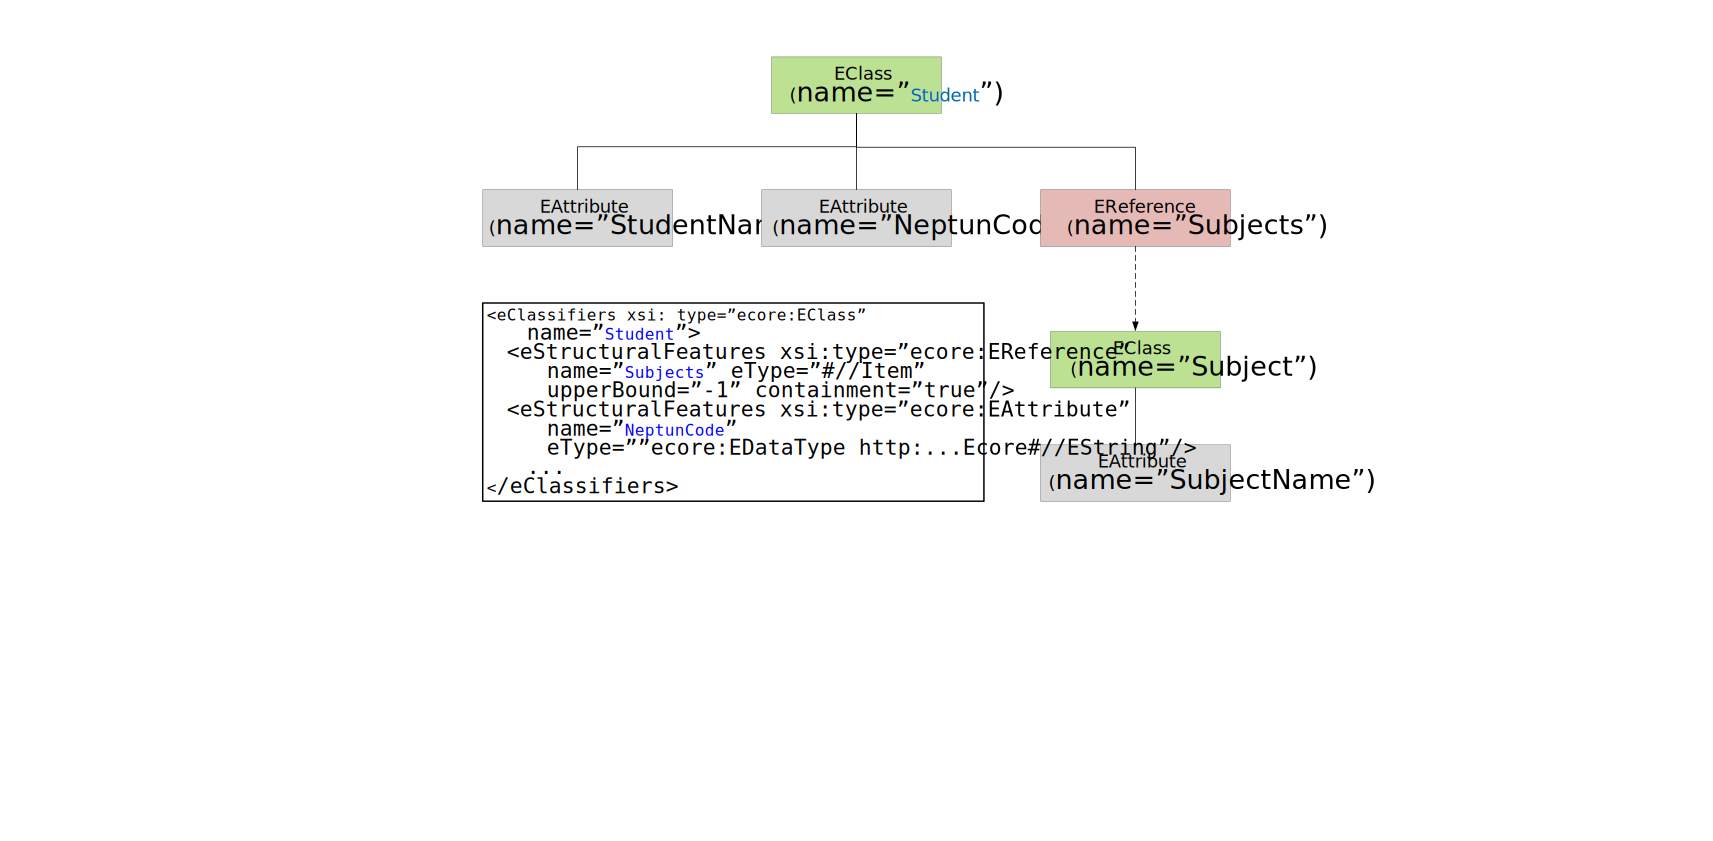
\includegraphics[width=\textwidth]{figures/datamodel-example-with-xmi-desc.pdf}
\caption{Ecore metamodell példa és XMI formátumú megadása}
\label{fig:DataModelWithXMI}
\end{figure}
%Az \gls{EMF} modell lényegében az UML osztálydiagram nézetének egy részhalmaza \cite{EMFFundamentals}.

Az Ecore metamodellek létrehozását az \ref{fig:EcoreDiagramEditor}. ábra szerinti grafikus szerkesztő segíti.
%
\begin{figure}[htb]
\centering
\includegraphics[width=\textwidth]{figures/ecore-diag-editor.png}
\caption{Ecore grafikus modellszerkesztő}
\label{fig:EcoreDiagramEditor}
\end{figure}
%
A \ref{fig:EcoreMetaModelExample}. ábra a szerkesztővel készíthető metamodellre mutat egy példát\footnote{Network modell. Forrás: \url{https://github.com/ujhelyiz/EMF-IncQuery-Examples/tree/master/network} (2014.05.21.)}.
%
\begin{figure}[htb]
\centering
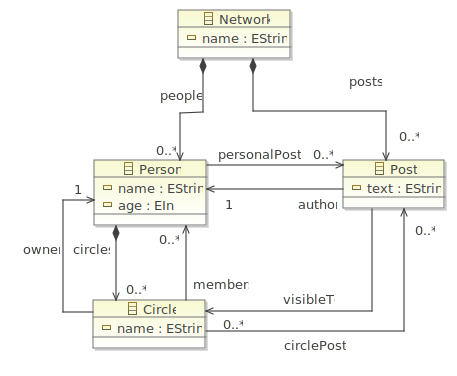
\includegraphics[width=\textwidth]{figures/ecore-network-metamodel-diag.pdf}
\caption{Példa grafikus szerkesztővel megadott Ecore metamodellre (Network modell)}
\label{fig:EcoreMetaModelExample}
\end{figure}
A \ref{fig:EcoreMetaModelExample}. ábrán látható diagram az \gls{UML} osztálydiagramjának nyelvezetét követi.
Megjelennek rajta az osztályokat szimbolizáló dobozok, azokban az osztály neve, illetve attribútumai névvel és típussal.
A dobozokat névvel és multiplicitással rendelkező élek kötik össze, melyek az osztályok közötti referenciákat jelzik.
A tartalmazást szimbolizáló éleken megjelenik az UML-ből ismert teli rombusz is.
Az \gls{EMF} modellek a grafikus szerkesztőn kívül az alábbi módokon is megadhatóak:
\begin{enumerate}
	\item Java Interfaces
	\item UML Class Diagram
	\item XML Schema
\end{enumerate}

A dolgozatban kulcsszerepet játszó Eclipse Modeling Framework (\gls{EMF}) bemutatásának összefoglalásaként a következőket emelhetjük ki \cite{EMFFundamentals}:
Az \gls{EMF} a legkézenfekvőbb modellező eszköz az Eclipse számára, mivel nagyszerűen beépül és együttműködik a környezettel és az azt körülvevő szoftver-ökoszisztémával.
A modellezést és a programozást keverten is képes kezelni növelve ezáltal mindkettő hatásfokát.
A szoftverfejlesztés termelékenységét növeli és megkönnyíti az integrációt.
Mindezek alapján az Eclipse modell alapú fejlesztésének és adatintegrációjának az alapja. 

A feladatkiírás szerint az \gls{EMF}-re épülő, a Budapesti Műszaki Egyetem Méréstechnika és Információs Rendszerek Tanszékének Hibatűrő Rendszerek Kutatócsoportja által kidolgozott, modell-lekérdezések végrehajtására alkalmas EMF-IncQuery keretrendszerben kell vizsgálatokat végeznem, ezért a következőkben ezt a keretrendszert ismertetem.

%----------------------------------------------------------------------------

\section{EMF-IncQuery}\label{sect:IncQuery}

A szekció célja bemutatni az EMF-IncQuery és a lekérdezőnyelv felépítését, használatát, továbbá, a feladatkiírás első pontjának megfelelően, a modell-lekérdezések fogalmát az EMF-IncQuery keretrendszeren keresztül.

A keretrendszer főbb tulajdonságait röviden a \cite{EMFIncQuery} foglalja össze:
Az EMF-IncQuery \gls{EMF} modelleken végzendő deklaratív lekérdezések definiálására és végrehajtására alkalmas keretrendszer.
Fontos jellemzője, hogy a definiált lekérdezéseket kézi programírás nélkül, hatékonyan hajthatjuk végre.
A lekérdezőnyelv a gráfminták matematikai formalizmusán alapul, amely tömör és egyszerű eljárás komplex szerkezetű modell-lekérdezések megadására.
A kiemelkedő futási teljesítményt azáltal nyújtja, hogy inkrementális gráfminta illesztési technikákat alkalmaz.
Ennek köszönhetően a keresést elég egyszer elvégezni, a továbbiakban a lekérdezés kiértékelése még milliós nagyságrendű elemszám mellett is gyors.
Emellett az \gls{EMF} pár hiányosságát is orvosolja, mint például az osztályok egyedinek gyors és hatékony felsorolása helyre való tekintet nélkül, egyszerű fordított navigáció bármilyen referencia mentén, és objektumok megkeresése attribútum érték alapján.
Az újabb verzió képes származtatott tulajdonságok -- virtuális attribútumok és referenciák -- kiértékelésére is.

\subsection{Felépítés}

Az EMF-IncQuery felépítését a \ref{fig:EMFIncQueryStructure}. ábra mutatja \cite{Bergmann-TOOLS-2012}.
%
\begin{figure}[htb]
\centering
\includegraphics[width=\textwidth]{figures/emf-incquery-structure.png}
\caption{Az EMF-IncQuery felépítése}
\label{fig:EMFIncQueryStructure}
\end{figure}
%
A megadott lekérdezésen (Query specification) alapulva mintaellenőrző pluginok generálódnak (Generated pattern matcher), melyek könnyen integrálhatók egy meglévő Eclipse-alapú alkalmazásba (Application, Application code).
A lekérdezés megadását Xtext 2-alapú szerkesztő támogatja, amely fejlett szintaxis kiemeléssel, kódkiegészítéssel és formula ellenőrzéssel rendelkezik.
Ezek a pluginok az EMF-IncQuery API-n keresztül elérik a rendszer belső funkcionalitását.
Az API-ban a Validation Engine, modell-helyesség ellenőrző motor körbeveszi az \gls{EMF} Validációs szolgáltatást (Validation Service), hogy EMF-IncQuery-alapú online jól formáltság ellenőrzőket nyújtson a szabványos Eclipse hiba-markerek révén.
Az interpretáló mintaillesztő (Interpretative pattern matcher) közvetlenül Java kódból indított ad-hoc lekérdezések gyors végrehajtásához nyújt elérési pontot.
Az API nyújtja továbbá a származtatott sajátosságok támogatását (Derived feature support).
A keretrendszerben a Base komponens gyakran használt alacsony szintű inkrementális lekérdezéseket nyújt, mint pl. a már említett egyed felsorolások, és fordított irányú navigálás egyirányú hivatkozásokon.
A lekérdezések inkrementális kiértékelését és életciklus kezelését a RETE motor szolgáltatja (RETE Core).
Az IncQuery Core adja az EMF-IncQuery keretrendszer magját.
A rendszer jellemzőinek mélyebb megértéséhez és az általa nyújtott szolgáltatások feltárásához a \cite{Bergmann-TOOLS-2012} irodalom volt segítségemre.

A gráfmintázatok keresése azzal az előnnyel jár, hogy a gráfminta által reprezentált feltételek vagy korlátozások a modellgráf megtalált, egyező mintázatú részén is teljesülnek.
A gráfminta strukturális, topológiai elvárásokat jelent, megadva az adott típusú élek és csomópontok kereséséhez az információt, továbbá kifejezésekkel az attribútumértékek iránt fogalmaz meg elvárásokat.
Egyes mintarészek/jellemzők kizárhatók az egyezés iránti elvárásból.
A gráfminta keresés ilyen módon nagyon finoman paraméterezett keresések kivitelezésére ad módot.

\subsection{Használat}

Ha egyszerűen csak használni szeretnénk az EMF-IncQuery által nyújtott szolgáltatásokat, akkor nem kell mást tennünk, mint telepíteni az EMF-IncQuery SDK-t, illetve a hiányzó függőségeket a már meglévő Eclipse környezetünkbe \cite{EclipseOrgIncQueryInstall}.
Ha azonban újabb komponenseket szeretnénk a keretrendszerhez fejleszteni, akkor a \cite{EclipseOrgIncQueryDevEnv} forrás lesz a segítségünkre.
A fejlesztés megkezdéséhez először le kell tölteni a keretrendszer forráskódját, majd importálni a projekteket a fejlesztői környezetünkbe.
Ezután, az Xtext kódgeneráló munkafolyamatainak (MWE2 szkriptek) végrehajtásával előbb legeneráljuk a lekérdezőnyelv feldolgozásához szükséges kódot, majd javasolt a projekt tisztítása és teljes újrafordítása.
Az eredményt Eclipse Application-ként futtatva, egy olyan Eclipse fejlesztői környezet indul el, amelybe automatikusan betöltődnek az EMF-IncQuery moduljai.

Az így kapott környezetben kipróbálhatjuk az EMF-IncQuery-t: írhatunk lekérdezéseket a tárgynyelven, majd lefuttathatjuk őket példánymodelleken.
Ehhez azonban szükségünk lesz egy modellre.
Ha rendelkezünk már megfelelő \gls{EMF} modellel, akkor használhatjuk azt, én azonban szeretném röviden bemutatni a modell elkészítésének menetét.

Mint modellezéskor mindig, most is egy domén specifikációjából fogunk kiindulni.
Az általam modellezett domén a karate harcművészetet űzők egy egyszerűsített világa lesz.
Ennek a világnak fő elemei a \emph{karatékák}, a karate harcművészek.
Minden karatékának van neve, és lehet egy meghatározott stílusa.
A karatékák lehetnek \emph{mesterek} vagy \emph{tanítványok}.
A tanítványok egy és csak egy mester alatt tanulhatnak, azonban a mestereknek nem szükségszerű, hogy legyen tanítványuk.
Minden mester a saját \emph{dódzsójában} (edzőterem, klub) oktatja tanítványait, melynek van neve.
Az előző két mondat állításaiból következik, hogy egy tanítvány egyszerre pontosan egy dódzsóban tanulhat.

Ezen leírás alapján elkészíthetjük a domén metamodelljét az \gls{EMF} Ecore diagram alapú modellezőjének segítségével.
Ennek mikéntjéről bővebb leírást a \cite{VogelEMF} ad.
Az általam elkészített metamodellt a \ref{fig:karateMetaModel}. ábra mutatja.
%
\begin{figure}[htb]
\centering
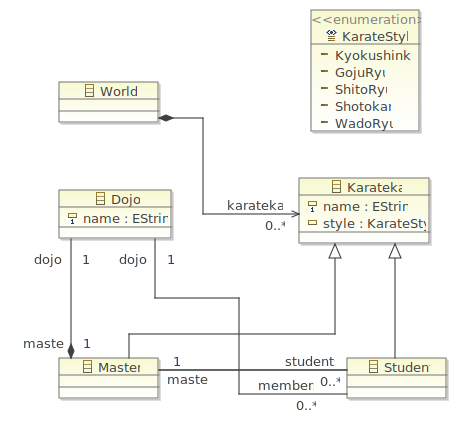
\includegraphics[width=\textwidth]{figures/ecore-karate-metamodel-diag.pdf}
\caption{Karate metamodell}
\label{fig:karateMetaModel}
\end{figure}
%
Az ábrán látható diagram az UML osztálydiagramok jelölésrendszerét használja.
Jól láthatóak a kapcsolatok a modell főbb elemei közt: a Master és Student osztályok leszármazottjai az absztrakt Karateka osztálynak, megjelennek kétirányú kapcsolatok a Master, Student és Dojo osztályok között.
A KarateStyle a lehetséges karate stílusok felsorolása.
A modell gyökere a World osztály, ez tartalmazza a Karateka-kat, akik közül a Master típusúak tartalmazzák a Dojo-kat.

Az Ecore metamodell alapján elkészíthetjük a Genmodel metamodellt, amelyből generálhatjuk a modellünk egyedeinek létrehozásához és manipulálásához szükséges Java kódot és az Eclipse-be beépülő szerkesztő komponenseket, melyek segítenek a példánymodellek vizuális konstrukciójában.
A következő lépésben az elkészült komponenseket -- az EMF-IncQuery komponenseivel együtt -- betöltjük az Eclipse környezet egy újabb példányába a már említett módon (futtatás Eclipse Application-ként).
Itt varázsló segítségével létrehozhatjuk a modellünk egy új egyedét, melyet feltölthetünk a szükséges tartalommal.
Én a példánymodellemet a \emph{The Karate Kid} (A karate kölyök) című 1984-es kultuszfilm alapján készítettem el, töltöttem fel adatokkal.
Az elkészült példánymodellt fa formában a \ref{fig:karateInstanceModel}. ábra mutatja.
%
\begin{figure}[htb]
\centering
\includegraphics[width=0.70\textwidth]{figures/karate-instance-tree-with-properties.png}
\caption{Karate példánymodell}
\label{fig:karateInstanceModel}
\end{figure}
%

Példánymodellünk kész, jöhet a keresés!
A kereséshez szükségünk lesz egy gráfmintára.
Egy egyszerű, az EMF-IncQuery lekérdezőnyelvén megadott mintát láthatunk a \ref{lst:isStudentOfMiyagiPattern}. kódlistán.
%
\begin{lstlisting}[float,floatplacement=htb,caption=isStudentOfMiyagi gráfminta a tárgynyelven,label=lst:isStudentOfMiyagiPattern]
package karate.incquery

import "http://karate/1.0"

pattern isStudentOfMiyagi(student : Student) = {
    Student.master.name(student, "Kesuke Miyagi");
}
\end{lstlisting}
%
Ha a mintát beregisztráljuk az EMF-IncQuery \emph{Query Explorer} nézetébe és betöltjük mellé a példánymodellünket (\ref{fig:karateInstanceModel}. ábra) is, akkor a lekérdezés automatikusan kiértékelődik, és a \ref{fig:karateQueryResult}. ábrán látható eredményt kapjuk.
%
\begin{figure}[htb]
\centering
\includegraphics[width=\textwidth]{figures/karate-query-result.png}
\caption{A keresés eredménye}
\label{fig:karateQueryResult}
\end{figure}

\subsection{A lekérdezőnyelv}

A \ref{lst:isStudentOfMiyagiPattern}. kódlistán bemutatott keresési minta az EMF-IncQuery saját, deklaratív gráfminták leírására szolgáló nyelvén (IncQuery Graph Pattern language, IQPL) íródott, mely szintaxisának jelentős részét a VIATRA2 Textual Command Language-ből (VTCL) örökli, szemantikája pedig hasonló a Datalog deklaratív logikai lekérdezőnyelvéhez \cite{Ceri:1989:YAW:627272.627357}.

A nyelv feldolgozását a már említett Xtext keretrendszer végzi, mely programozási és doménspecifikus nyelvek fejlesztéséhez nyúlt alapot: az elemzéstől, a fordításon keresztül, a teljes Eclipse integrációig lefedi a szükséges nyelvi infrastruktúrát.
Az Xtext biztosít olyan eszközöket is, mint a szintaxis kiemelés, a kontextus alapú kiegészítés vagy a validáció.

A nyelv a következő fontosabb elemekből épül fel \cite{EclipseOrgIncQueryLang}:
\begin{description}
\item[Csomag:] a \texttt{package} direktíva -- a Java-hoz hasonlóan -- jelzi, hogy melyik csomag tartalmazza a fájlban lévő mintákat
\item[Importok:] \texttt{import} direktívákkal adhatjuk meg azokat az \gls{EMF} csomagokat, melyeknek elemeire hivatkozni szeretnénk a lekérdezésekben
\item[Minta:] a \texttt{pattern} kulcsszóval bevezetett minták olyan \emph{predikátumok}, melyeknek lehetnek paramétereik -- melyeknek opcionálisan megadhatjuk a típusát is --, annotációik, és legalább egy törzsük van; a minta törzsei logikai VAGY kapcsolatban, vagyis diszjunkcióban állnak egymással
\item[Mintatörzs:] a kapcsos zárójelek által határolt mintatörzs legalább egy kényszerből és valahány lokális változóból áll; a törzsben lévő kényszerek logikai ÉS kapcsolatban állnak egymással 
\item[Kényszer:] kényszerek segítségével adhatóak meg a változók tulajdonságai és a közöttük lévő kapcsolatok; egy vagy több változóhivatkozás található bennük
\item[Változó:] értéke megadható, vagy mintaillesztésnél helyettesítődik be; a minta paramétereit \emph{paraméterváltozóknak}, a csak a törzsekben találhatóakat pedig \emph{lokális változóknak} nevezzük; a lokális változók első említésükkor impliciten deklarálódnak
\item[Annotáció:] a mintához kapcsolható metaadat; szintaxisa és szemantikája a Java nyelv annotációit követi
\end{description}

A \ref{lst:isStudentOfMiyagiPattern}. kódlistán a nyelv szinte minden elemére találhatunk példát.
Az kód 1. sora jelzi, hogy a minta a \texttt{karate.incquery} csomag része.
A 3. sorban a \texttt{http://karate/1.0} névtér importálása történik, melyre a \texttt{Student} típus használatához van szükség.
Az 5-7. sor definiálja az \texttt{isStudentOfMiyagi} nevű mintát, melynek egy \texttt{student} névre hallgató paramétere van.
A \texttt{student} paraméterváltozó típusa (\texttt{Student}) expliciten van megkötve a paraméterlistán.
A minta -- esetünkben egyetlen -- törzse az egyenlőségjel utáni nyitó, és a kód végén található záró kapcsos zárójelek közötti rész.
Itt találhatóak a mintatörzs kényszerei, amiből esetünkben csak egy van.
A \texttt{Student.master.name(student, "Kesuke Miyagi")} kényszer egy útvonal-kifejezés kényszer (path expression constraint), mely azt a feltételt fejezi ki, hogy a \texttt{student} változóba csak olyan érték kerülhet, amely egyrészt \texttt{Student} típusú, másrészt a \texttt{master} tulajdonságának a neve (\texttt{name} tulajdonságának értéke) a \textit{``Kesuke Miyagi''} sztring.

A keresőminta egy törzse akkor \emph{illeszkedik}, ha sikerül olyan változóbehelyettesítést találni, amelyre a törzsben található kényszerek ki vannak elégítve.
Maga a keresőminta pedig akkor illeszkedik, ha paraméterváltozóinak van olyan behelyettesítése, melyre legalább az egyik törzse illeszkedik.

A fentiek alapján a \ref{lst:isStudentOfMiyagiPattern}. kódlistán látható keresőminta a \ref{fig:karateInstanceModel}. ábrán látható példánymodell egyetlen elemére illeszkedik, ahogyan azt a találati eredmények is mutatják (\ref{fig:karateQueryResult}. ábra).

A nyelvben az eddig bemutatottal együtt összesen öt kényszertípus található, melyet az alábbi szekciók mutatnak be röviden.

\subsubsection{Ellenőrzés kényszer (check constraint)}
Ez a kényszer egy tetszőleges, igaz-hamis értékű Java kifejezést értékel ki a paramétereire.
Ajánlott a kifejezésnek mellékhatás mentesnek lennie, mivel csak ekkor garantálható a helyes működés \cite{EclipseOrgIncQueryLang}.

\noindent Általános formája: \texttt{check(\textit{<Java kifejezés>})}

\noindent Példa:
\begin{lstlisting}
package karate.incquery

import "http://karate/1.0"

pattern overlongStyles(style : KarateStyle) = {
    check(style.literal.length > 10);
}
\end{lstlisting}
    
\subsubsection{Összehasonlítás kényszer (compare constraint)}
Ez a kényszer a jobb és bal oldalán álló két kifejezés egyenlőségét vagy egyenlőtlenségét fejezi ki.

\noindent Általános formája:
\begin{description}
\item[egyenlőség:] \texttt{\textit{<kifejezés>} == \textit{<kifejezés>}}
\item[egyenlőtlenség:] \texttt{\textit{<kifejezés>} != \textit{<kifejezés>}}
\end{description}

\noindent Példa:
\begin{lstlisting}
package karate.incquery

import "http://karate/1.0"

pattern stylesOtherThanGojuRyu(style : KarateStyle) = {
    style != KarateStyle::GojuRyu; 
}
\end{lstlisting}
    
\subsubsection{Típuskényszer (EClassifier constraint)}
Ez a kényszer a paraméterének típusát határozza meg.
Azt már láttuk, hogy egy minta paraméterváltozójának típusát megadhatjuk explicit módon a paraméterlistán.
Ez a megadás azonban egy ekvivalens típuskényszer alkalmazásával helyettesíthető.
A lokális változók típusának explicit megkötésére a típuskényszer a legalkalmasabb eszköz, ám még így is viszonylag ritkán fordul elő, mivel egy változó típusa az egyéb kényszerekben betöltött szerepe alapján általában kikövetkeztethető.

\noindent Általános formája: \texttt{\textit{<típus>}(\textit{<változó>})}

\noindent Példa:
\begin{lstlisting}
package karate.incquery

import "http://karate/1.0"

pattern masters(karateka) = {
    Master(karateka);
}
\end{lstlisting}

\subsubsection{Útvonal-kifejezés kényszer (path expression constraint)}
Ez a kényszer két paramétere egy vagy több modell-élen keresztüli kapcsolatát fejezi ki.
A kényszer ennek megfelelően egy fejből, és egy vagy több farokból áll.
A fej egy típus, és a kényszer első paraméterének típusát határozza meg.
Az első farok a fej egy tulajdonsága (attribútuma vagy referenciája), mely szintén meghatároz egy típust: a tulajdonság típusát.
A következő farok -- ha van -- ennek a típusnak egy tulajdonsága, és így tovább a további farkakra.
Az utolsó farok a kényszer második paraméterét határozza meg.

\noindent Általános formája: \texttt{\textit{<típus>}.\textit{<él$_1$>}.$\cdots$.\textit{<él$_n$>}(\textit{<kifejezés>}, \textit{<kifejezés>})}

\noindent Példa: lásd \ref{lst:isStudentOfMiyagiPattern}. kódlista

\subsubsection{Minta kompozíciós kényszer (pattern composition constraint)}
Ez a kényszer egy már meglévő minta felhasználását, úgymond \emph{hívását} teszi lehetővé.
A kényszer akkor teljesül, ha a felhasznált minta illeszkedik a paramétereire.
A minta hívása lehet \emph{negatív} (negative application condition, \gls{NAC}) is, amit a \texttt{neg} prefix jelez.
Ebben az esetben a kényszer akkor teljesül, amikor a minta nem illeszkedik a paramétereire.

\noindent Általános formája: \texttt{\textit{[}neg\textit{]} find \textit{<minta>}(\textit{<kifejezés$_1$>}, $\cdots$, \textit{<kifejezés$_n$>})}

\noindent Példa -- a már megismert \texttt{isStudentOfMiyagi} minta tölti be a meglévő minta szerepét:
\begin{lstlisting}
package karate.incquery

import "http://karate/1.0"

pattern isStudentOfMiyagi(student : Student) = {
    Student.master.name(student, "Kesuke Miyagi");
}

pattern notStudentOfMiyagi(student : Student) = {
    neg find isStudentOfMiyagi(student);
}
\end{lstlisting}

\vspace{\baselineskip}\noindent % section continuation hack
A kényszerek paramétereiként megjelenő kifejezések -- kivéve az ellenőrzés kényszer Java kifejezéseit -- négy különböző formában jelennek meg:
\begin{description}
    \item[változóreferencia:] hivatkozás egy lokális vagy paraméterváltozóra; 
    \item[érték literál:] lehet igaz-hamis érték, egész szám, lebegőpontos szám, vagy szöveg, illetve kifejezések egy listája (\texttt{\{\textit{<kifejezés$_1$>}, $\cdots$, \textit{<kifejezés$_n$>}\}})
    \item[felsorolható típus literál:] hivatkozás felsorolt típus (enum) elemére; egy példát az összehasonlítási kényszer leírásánál találhatunk rá (\texttt{KarateStyle::GojuRyu})
    \item[aggregátor kifejezés:] ez a kifejezés egy érték származtatását teszi lehetővé a minta változóinak függvényében; két típusa létezik:
    \begin{itemize}
        \item a \texttt{count} kifejezés egy minta illeszkedéseinek számát adja vissza; szintaxisa: \mbox{\texttt{count find \textit{<minta>}(\textit{<kifejezés$_1$>}, $\cdots$, \textit{<kifejezés$_n$>})}}
        \item \begin{sloppypar}az \texttt{eval} kifejezés egy tetszőleges Java kifejezést értékel ki; szintaxisa: \mbox{\texttt{eval(\textit{<Java kifejezés>})}}\end{sloppypar}
    \end{itemize}
\end{description}

A lokális változók egy speciális esete az \emph{egyszer használatos változó}.
Ilyen változót abban az esetben használunk, ha a változó értéke számunkra lényegtelen, de a szintaxis megkívánja egy változó jelenlétét.
Az ilyen változókra mintatörzsenként pontosan egy hivatkozás lehet.
Ezek a változók onnan ismerhetőek fel, hogy nevük egy alulvonással kezdődik, például \texttt{\_dontcare}.
Egy speciális eset az \emph{anonim változó}, amelyre egy alulvonás karakterrel (\texttt{\_}) tudunk hivatkozni.
Ez többször is szerepelhet egy törzsön belül, ám minden említése egyedi változónak számít.
